\documentclass[25pt, a0paper, portrait, blockverticalspace=.5cm]{tikzposter}
\usepackage[utf8]{inputenc}
\usepackage{amssymb,amsfonts,amsmath,mathtext,mathtools}
\usepackage{xfrac}
\usepackage{enumitem}

\let\vec\oldvec
\newcommand{\vec}[1]{\boldsymbol{#1}}

\title{\parbox{\linewidth}
	{\centering
		Longitudinal dynamic in NICA Barrier Bucket RF System at transition energy including impedances in BL\MakeLowercase{on}D\		
}}

\author{S. Kolokolchikov\textsuperscript{1, 2}*, Y. Senichev\textsuperscript{1, 2}, A. Aksentyev\textsuperscript{1, 2, 3}, \\A. Melnikov\textsuperscript{1, 2, 4}, 
		E. Syresin\textsuperscript{5}, V.Ladygin\textsuperscript{5}}
\institute{
	\textsuperscript{1} Institute for Nuclear Research (RAS), Moscow, Russia,\\
	\textsuperscript{2} Moscow Institute of Physics and Technology, Dolgoprudny, Russia,\\
	\textsuperscript{3} Moscow Engineering Physics Institute, Moscow, Russia,\\
	\textsuperscript{4} Landau Institute for Theoretical Physics (RAS), Chernogolovka, Russia,\\
	\textsuperscript{5} Joint Institute for Nuclear Research, Dubna, Russia\\
	*sergey.bell13@gmail.com
}
\usetheme{Simple}
\usecolorstyle{Russia}
\colorlet{blocktitlefgcolor}{black}

\usepackage{caption}
\captionsetup{font=large}
\usepackage{multicol}
\setlength\columnsep{1.5cm}

\begin{document}

\maketitle


\begin{columns}
\column{.56}

\block{INTRODUCTION}{

\par At an experiment on acceleration of a polarized proton beam up to an energy at 13 GeV, the possibility of crossing the transition energy at 5.7 GeV by a jump is considered. The scheme of crossing by a rapid change of transition energy, assumes the longitudinal movement of the beam near the zero value of the slip-factor. The jump itself is carried out in the absence of an RF field. 

\par The paper investigates the impedance influence on longitudinal dynamics during the procedure of transition energy crossing with a jump. A distinctive feature is the use of Barrier Bucket RF, as a result a specific distribution of the beam in the phase space, different from the classical one, formed by harmonic RF.
}
\block{$\gamma$-TRANSITION JUMP}
{
\begin{minipage}{0.55\linewidth}
	\par Equations of longitudinal motion describe a particle evolution in phase space. And at transition is necessary to consider high orders $\eta = \eta_{0}+\eta_{1} \delta$, differs for each particle.
\end{minipage}
\begin{minipage}{0.45\linewidth}
		\begin{equation}
		\begin{aligned}
		& \frac{d \tau}{dt}=\eta (\delta) \cdot \frac{h \cdot \Delta E}{\beta^2 \cdot E_0} \\
		& \frac{d(\Delta E)}{dt}=\frac{V(\tau)}{T_0}
		\end{aligned}
		\end{equation}
\end{minipage}

\begin{minipage}{0.55\linewidth}
	\par Longitudinal dynamics states based on $\gamma_{tr}$ change:\\
\par 1) acceleration from $E_{inj}$ with stationary value;
\par 2) smooth increase parallel with $\gamma$-particle to peak, slip-factor $\eta_0$ gets the minimal possible value;  
\par 3) jump over stationary value of transition, as soon as $\eta_0$ flipping over $0$ value for all particles;
\par 4) smooth recovery to stationary $\gamma_{tr}$;
\par 5) acceleration till the experiment energy;\\

\par States 2-3-4 defines the $\gamma_{tr}$-jump procedure. To maintain, the magneto-optics changed by quadrupole gradients variation. This lead to dependance of $\gamma_{tr}$ and tunes $\nu_{x,y}$. Stability region defines by dynamic aperture.
\end{minipage}
\begin{minipage}{0.45\linewidth}
	\begin{tikzpicture}
	\node (cone) at (0,0) {\includegraphics[width=\linewidth]{TEXPaper/img/fig_01.png}};
	\end{tikzpicture}
\end{minipage}

		\begin{minipage}{0.5\linewidth}
			\begin{tikzpicture}
			\node (cone) at (0,0) {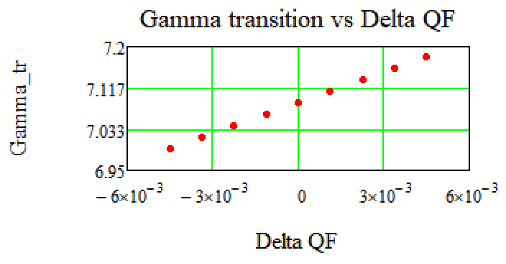
\includegraphics[width=\linewidth]{TEXPaper/img/fig_02-1.png}};
			\end{tikzpicture}
		\end{minipage}
		\begin{minipage}{0.5\linewidth}
			\begin{tikzpicture}
			\node (cone) at (0,0) {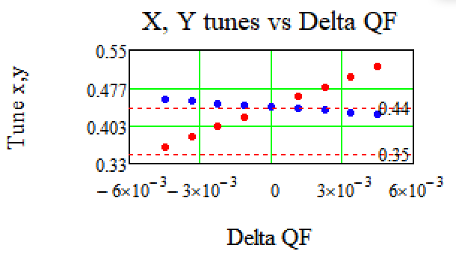
\includegraphics[width=\linewidth]{TEXPaper/img/fig_02-2.png}};
			\end{tikzpicture}
		\end{minipage}		
}	

\block{Barrier Bucket}{

		\begin{minipage}{0.47\linewidth}
			\begin{tikzpicture}
			\node (cone) at (0,0) {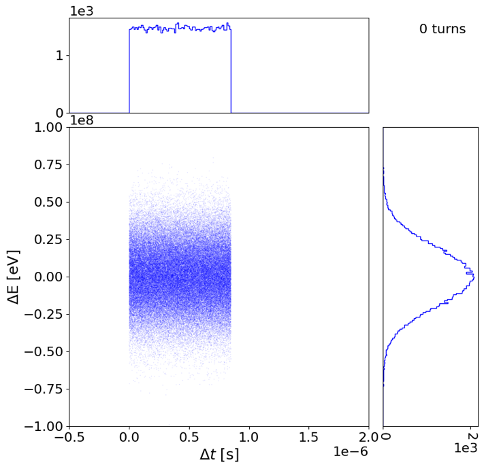
\includegraphics[width=\linewidth]{TEXPaper/img/fig_09-1.png}};
			\end{tikzpicture}
		\end{minipage}
		\begin{minipage}{0.47\linewidth}
			\begin{tikzpicture}
			\node (cone) at (0,0) {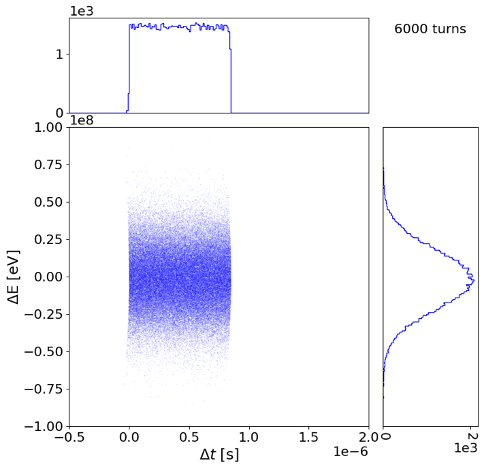
\includegraphics[width=\linewidth]{TEXPaper/img/fig_09-2.png}};
			\end{tikzpicture}
		\end{minipage}
		
		\begin{minipage}{0.5\linewidth}
		\end{minipage}
		
		\begin{minipage}{0.5\linewidth}
			
			\par Square Barrier Bucket RF signal fourier expansion.
			\begin{equation}
			b_n=\operatorname{sign}(\eta) \frac{2}{n \pi}\left[1-\cos \left(\frac{n}{h_{\mathrm{r}}} \pi\right)\right]
			\end{equation}
		 	\par Sigma-modulation make final signal smooth.
			\begin{equation}
			\sigma_{m, n}=\operatorname{sinc}^m \frac{n \pi}{2(N+1)}
			\end{equation}
		\end{minipage}
		\begin{minipage}{0.5\linewidth}
			\par Voltage amplitude for each term.
			\begin{equation}
			V_n=V^{\mathrm{peak}} b_{n} \sigma_{m, n}.
			\end{equation}
			\par Energy gain due to RFs kick. [1, 2]
			\begin{equation}
			\Delta E_i^{\prime}=\Delta E_i+\sum_{i=1}^{n_{\mathrm{rf}}-1} V_j \sin \left(\omega_j \Delta t_i+\phi_j\right)
			\end{equation}
		\end{minipage}
		

}
	
\column{.44}
	\block{TRACKING}{
	
	\section*{Before jump}

		\begin{minipage}{0.5\linewidth}
			\begin{tikzpicture}
			\node (cone) at (0,0) {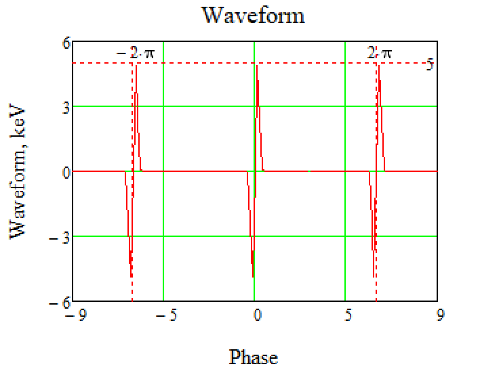
\includegraphics[width=\linewidth]{TEXPaper/img/fig_05-1.png}};
			\end{tikzpicture}
		\end{minipage}
		\begin{minipage}{0.5\linewidth}
			\begin{tikzpicture}
			\node (cone) at (0,0) {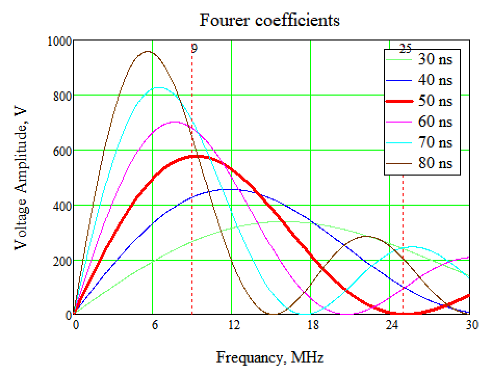
\includegraphics[width=\linewidth]{TEXPaper/img/fig_05-2.png}};
			\end{tikzpicture}
		
\end{minipage}
		\par Acceleration before jump itself lasts for about $2\times 10^5$ turns with RF focusing. And change polarity after jump. [3]

	\section*{During jump}
		\begin{minipage}{0.5\linewidth}
		\par In considered case, space charge impedance plays a dominant role.
		\newline
		\begin{equation}
		\frac{Z_{SC}}{n}=-\frac{Z_0\left[1+\log \left(\frac{b}{a}\right)\right]}{2 \beta \gamma^2}
		\end{equation}
		\par Due to special longitudinal distribution in Barrier Bucket, additional voltage 
		produced by SC influence only on particles at the edge [4]. And don't make any distortion during jump without RF.
		\end{minipage}
		\begin{minipage}{0.5\linewidth}
			\begin{tikzpicture}
			\node (cone) at (0,0) {\includegraphics[width=\linewidth]{TEXPaper/img/fig_04.png}};
			\end{tikzpicture}
		\end{minipage}

		\begin{minipage}{0.5\linewidth}
			\begin{tikzpicture}
			\node (cone) at (0,0) {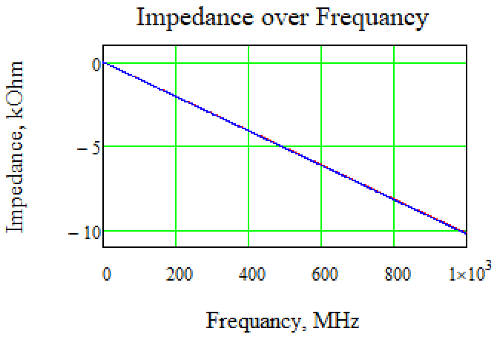
\includegraphics[width=\linewidth]{TEXPaper/img/fig_06-1.png}};
			\end{tikzpicture}
		\end{minipage}
		\begin{minipage}{0.5\linewidth}
			\begin{tikzpicture}
			\node (cone) at (0,0) {\includegraphics[width=\linewidth]{TEXPaper/img/fig_06-2.png}};
			\end{tikzpicture}
		\par 
			
\end{minipage}
\par RF is swiched off during jump ($6\times10^3$ turns) not to make any distortion, because particles move with different $\eta$, moreover, with various signs.


}

	\block{CONCLUSION}{
\par During the jump procedure the beam hold in separatrix. It helps to overcome the zero-value of slip-factor and don't lose beam. Jump procedure seems an available option cross transition energy.
}

	\block{REFERENCES}{
	 
	\par [1] Mihaly Vadai, Beam Loss Reduction by Barrier Buckets in the CERN Accelerator Complex, CERN, Geneva, 2021
	\par [2] A. Tribendis and others, Constraction and first test results of the barrier and harmonic RF systems for the NICA collider, IPAC2021, Campinas, SP, Brazil, doi:10.18429/JACoW-IPAC2021-MOPAB365
	\par [3] BLonD: https://blond.web.cern.ch/
	\par [4] J. Wei and S. Y. Lee, Space Charge Effect at Transition Energy and the Transfer of R.F. System at Top Energy, BNL-41667
	
	}
	
\end{columns}

\end{document}